% Ch5.tex

\chapter[Adaptive frequency scaled wavelet packet decomposition for frog call classification]{Adaptive frequency scaled wavelet packet decomposition for frog call classification}
\label{cha:cha5Wavelet}


\section{Introduction}
This chapter presents a novel cepstral feature representation based on adaptive frequency scaled wavelet packet decomposition. Following the conclusion of chapter 4 that cepstral features can achieve a good classification accuracy, but sensitive to the backgound noise, this research aims to develope a ceptral feature representation with a good anti-noise ability.



Since this thesis will address the low SNR recordings rather than high SNR recordings, developing feature representations with a good anti-noise ability is important. Different from most previous studies that extracted features using the Fourier transform, wavelet packet decomposition is employed in this study for feature extraction. The classsification performance is evaluated with two different datasets from Queensland, Australia (18 frog species from commercial recordings (high SNR) and field recordings of 8 frog species from James Cook University recordings (low SNR)). This chapter answers the research question 2(b): How to improve the performance of developed features for frog call classification in low SNR recordings? 


Although low SNR recordings are used in this reserach, we still regard the classification task as a single-instance single-label learning problem.
However, most low SNR recordings have more than one frog species. Therefore, in the next two chapters, we focus on the classification of multiple frog species in one individual recording.





\section{Journal paper - }


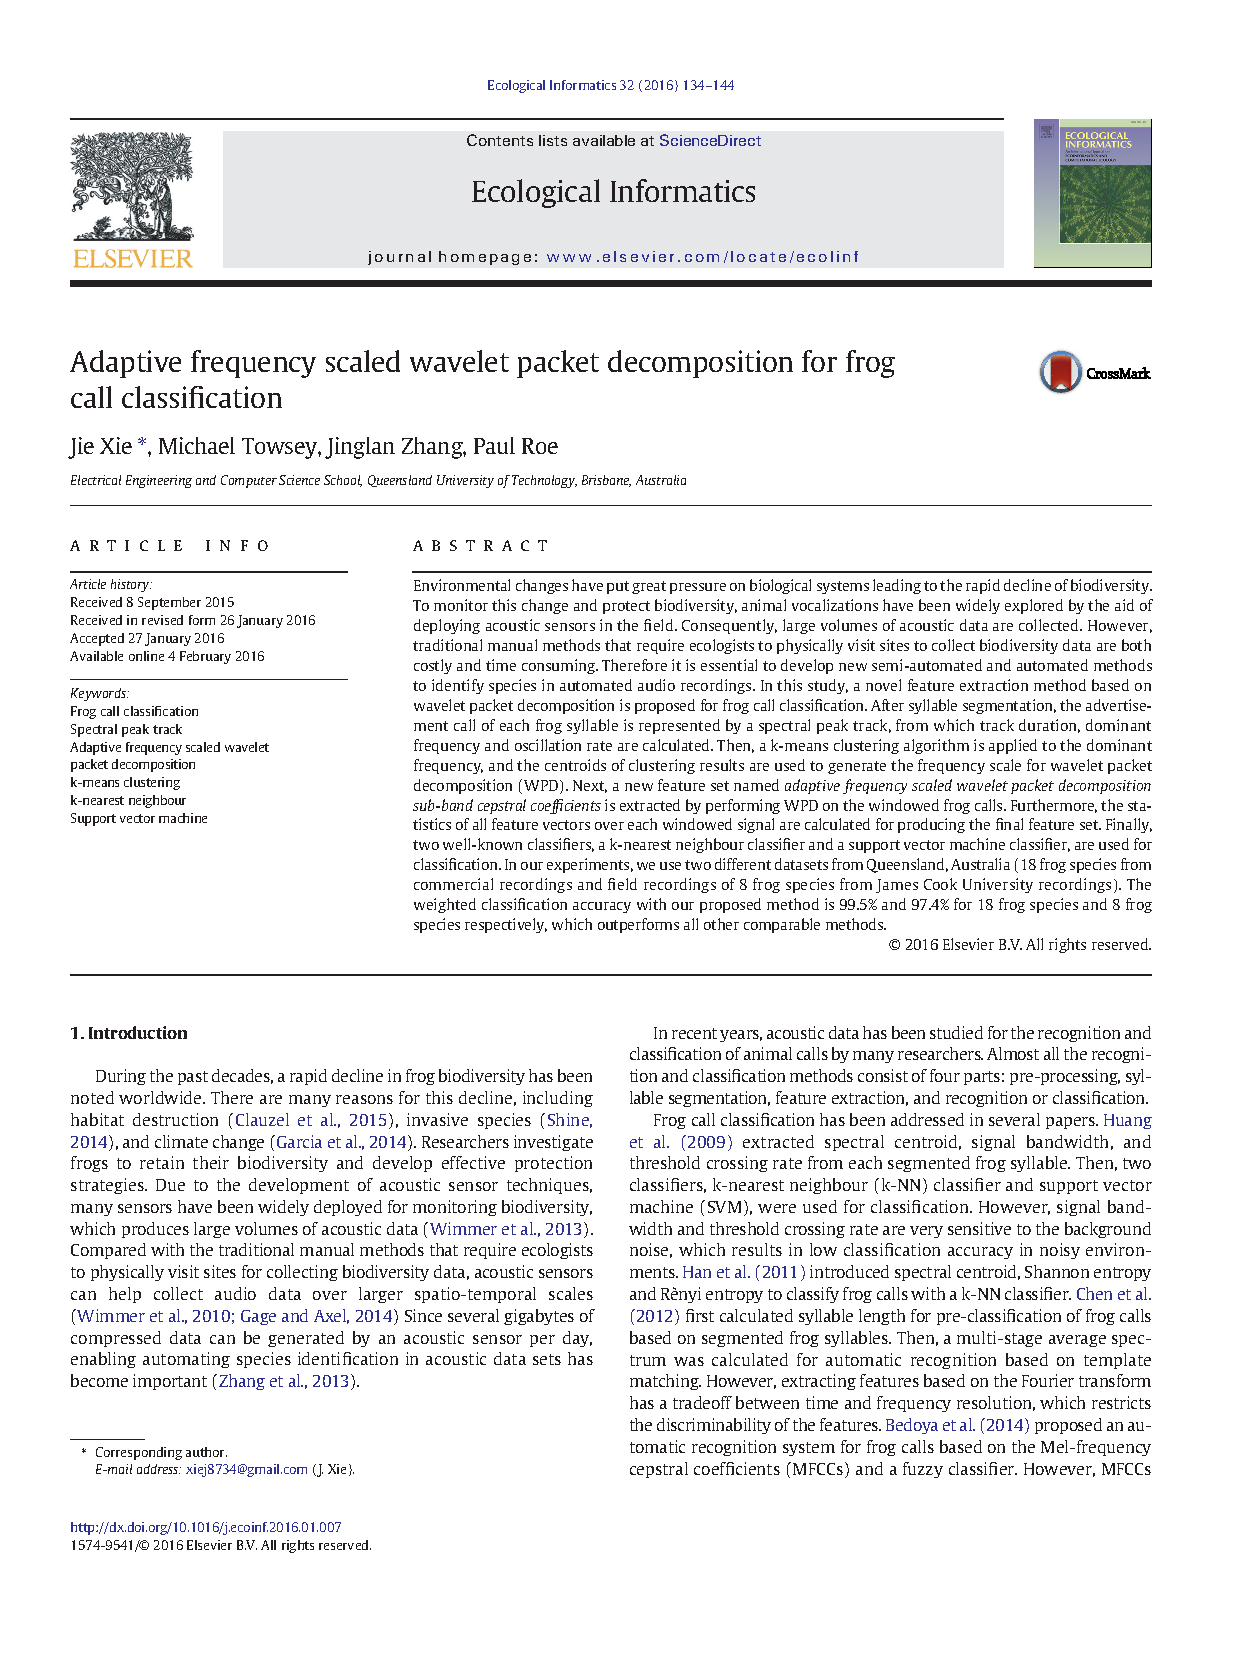
\includepdf[pages=-, pagecommand={},width=1.2\textwidth]{Ch5_paper.pdf}


